%\documentclass[12pt,a4paper,oneside]{reportu}
\documentclass[letterpaper, oneside, 12pt, these, creativecommons]{thETS}
\usepackage{times}
\usepackage[pdftex]{graphicx}
\usepackage{multirow}
\usepackage{pdfpages}
\usepackage{amsmath}
\usepackage{amssymb}
\usepackage{caption}
\usepackage[utf8]{inputenc}
\usepackage[frenchb]{babel}
\usepackage{amsmath}
\usepackage{caption}
\usepackage{multibib}
\usepackage{url}
\urlstyle{rm}

\begin{document}

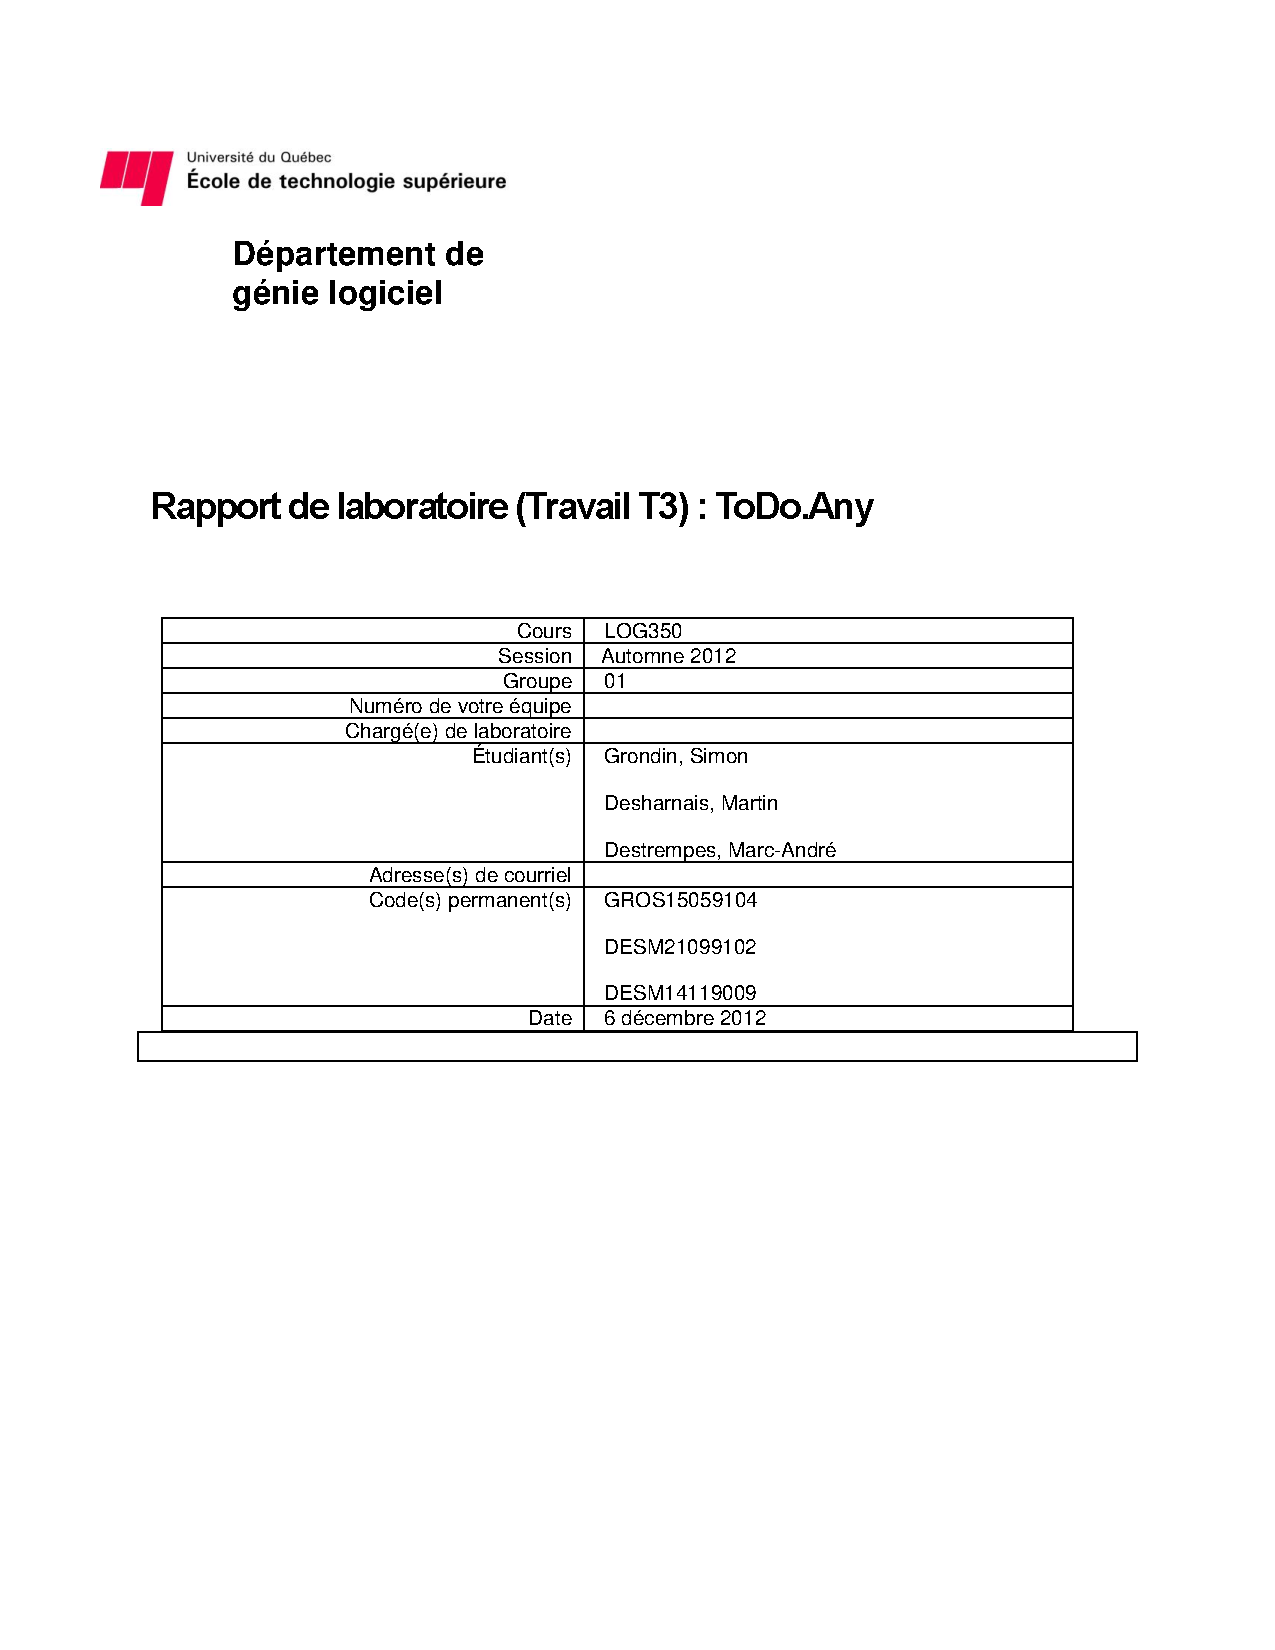
\includepdf[pages=-]{pageTitre.pdf}

\tableofcontents
\listoftables
\listoffigures

\chapter{Glossaire}

\begin{description}
\item[C\#] est un langage de programmation orienté objet à typage fort, créé par la société Microsoft. \footnote{\url{https://fr.wikipedia.org/wiki/C_sharp}}
\item[Windows Presentation Foundation] est la spécification graphique de Microsoft .NET 3.0. Il intègre le langage descriptif XAML qui permet de l'utiliser d'une manière proche d'une page HTML pour les développeurs. \footnote{\url{https://fr.wikipedia.org/wiki/Windows_Presentation_Foundation}}
\item[WinForms] est le nom de l'interface graphique qui est incluse dans .NET Framework, fournissant l'accès via du Managed code à l'API Windows. \footnote{\url{https://fr.wikipedia.org/wiki/Windows_Forms}}
\item[framework] est un kit de composants logiciels structurels, qui sert à créer les fondations ainsi que les grandes lignes de tout ou d’une partie d'un logiciel (architecture). \footnote{\url{https://fr.wikipedia.org/wiki/Framework}}
\item[.NET 4.5] est un framework pouvant être utilisé par un système d'exploitation Microsoft Windows et Microsoft Windows Mobile depuis la version 5 (.NET Compact Framework). \footnote{\url{https://fr.wikipedia.org/wiki/Framework_.NET}}
\item[SQLite] est une bibliothèque écrite en C qui propose un moteur de base de données relationnelle accessible par le langage SQL.\footnote{\url{https://fr.wikipedia.org/wiki/SQLite}}
\end{description}

\chapter{Introduction et sommaire du travail effectué en TP2}

L'application permet la gestion simple de tâches et d'événements tout en offrant des fonctionnalités de gestion et de classification avancées. Parmi celles-ci, notons la possibilite de définir des rappels, de catégoriser les éléments, de définir un événement comme échéance d'une tâche ou encore de définir des sous-tâches à une tâche imposante.

Durant notre analyse de tâche, nous avons déterminer que le publique cible est des personnes de 15 ans et plus désirant organiser son temps et sa vie professionnelle. De plus, nous avons conclu que notre interface devrais ressembler à des interfaces connu pour la garder familière et garder une courbe d'apprentissage faible. Pour ce faire, nous avons dressé une liste des cas d'utilisation que l'application doit traiter pour se donner un point de départ. Par la suite, nous avons construit nos prototypes statiques.

Pour construire notre prototype statique, nosu avons utilisé des fenêtres virtuelles où chaque point de chaque fenêtre à été détaillé pour s'assurer que le travail devant être effectué par chaque interface a bel et bien été compris. De plus, chaque fonctionnalité a aussi été détaillé dans le but qu'elles soient bien comprise.

Jusqu'à présent, presqu'aucune modification n'a été apporté entre les prototypes statiques et dynamiques. Tout va rester comme indiqué dans le document se trouvant à l'annexe III.

Dans le présent document, les tests qui seront effectués avec des utilisateurs seront listés et détaillés. Par la suite, un concensus sera fais pour chaque tâche et une amélioration qui pourrait être faite sera proposé pour améliorer le comportement du logiciel.

\chapter{Planification du travail}

\begin{table}
	\centering
	\begin{tabular}{|l|l|}
		\hline
		Semaine	& Travail accomplis 								\\ \hline
		4 novembre	& Choix de la technologie et apprentissage de celle-ci.		\\ \hline
		11 novembre	& Marc-André : Conception des interfaces. 				\\
				& Martin : Conception de la base de données.				\\
				& Simon : Conception de la base de données.				\\ \hline
		18 novembre	& Marc-André : Début de la rédaction du rapport. 			\\ 
				& Martin : Programmation du prototype dynamique. 			\\
				& Simon : Programmation du prototype dynamique. 			\\ \hline
		25 novembre	& Marc-André : Rédaction du rapport.		 			\\
				& Martin : Programmation du prototype dynamique. 			\\ 
				& Simon : Programmation du prototype dynamique.		 	\\ \hline
		2 decembre	& Marc-André : Rencontre avec les utilisateurs. 			\\
				& Martin : Rédaction du rapport.						\\
				& Simon : Rédaction du rapport.						\\ \hline
		9 decembre	& Marc-André : Préparation de la présentation.	 		\\ 
				& Martin : Préparation de la présentation.	 			\\ 
				& Simon : Préparation de la présentation.	 			\\ \hline
	\end{tabular}
	\caption{Échéancier}
\end{table}

\chapter{Réalisation du prototype dynamique}

Dans la section suivante, nous vous présenterons notre prototype dynamique et donc, avant d'entreprendre la lecture de cette section, nous vous conseillons de lire le document se trouvant à l'annexe III. Ce document contient les informations concernant le prototype statique et toute la logique derriere le prototype dynamique.

\section{Choix des outils}

Pour réaliser le prototype dynamique, nous avons décidé d'utiliser le C\# et le Windows Presentation Foundation (WPF) comme langages de programmation. Nous avons choisi ces langages tout simplement parce que ceci nous permet de séparer le code des interfaces et que le WPF va ultimement remplacer WinForms. 

Comme environnement de développement, nous utilisons Visual Studio 2012 avec le framework .NET 4.5 pour faciliter et accélérer notre développement. Ce framework nous donne des composantes graphiques de base qui nous simplifie la vie en nous permettant d'économiser du temps pour ne pas à avoir à developper des composants de base comme un TextBox ou un Label, par exemple.

De plus, comme base de données, nous utilisons SQLite parce que cela nous permet d'avoir un endroit pour stocker nos données de façon structuré et le tout dans un seul et unique fichier.

Pour assurer la gestion des versions, nous utilisons un logiciel connu sous le nom de Git. Ce logiciel s'occupe de faire la gestion des versions de chaque fichier du projet.

Pour la production de la documentation, nous utilisons le processeur de texte \LaTeX.

\newpage

\section{Captures d'écran}

\subsection{Fenêtre principale}

\newpage

\subsection{Événement}

C'est à partir de cette écran que l'utilisateur peut modifier ou créer un événement. À partir de cet écran, l'utilisateur peut aussi faire la gestion des alertes appartenant à l'événement. À la page 21 du document, dans l'annexe III, il y a de plus ample informations concernant cette fenetre.

\begin{figure}[H!]
	\centering
	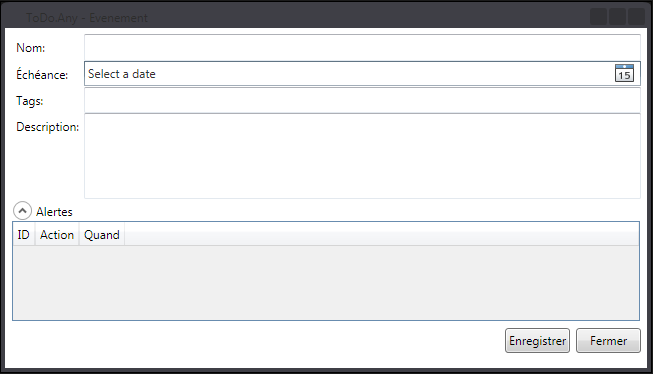
\includegraphics[width=1\textwidth]{fenetre_evenement.png}
	\caption{Fenêtre concernant un événement.}
\end{figure}

\newpage

\subsection{Tâche}

C'est à partir de cet écran que l'utilisateur peut modifier ou créer une tâche. À partir de cet écran, l'utilisateur peut aussi faire la gestion des alertes et des sous-tâches appartenant à la tâche parent. À la page 19 du document, dans l'annexe III, il y a de plus ample informations concernant cette fenêtre.

\begin{figure}[H!]
	\centering
	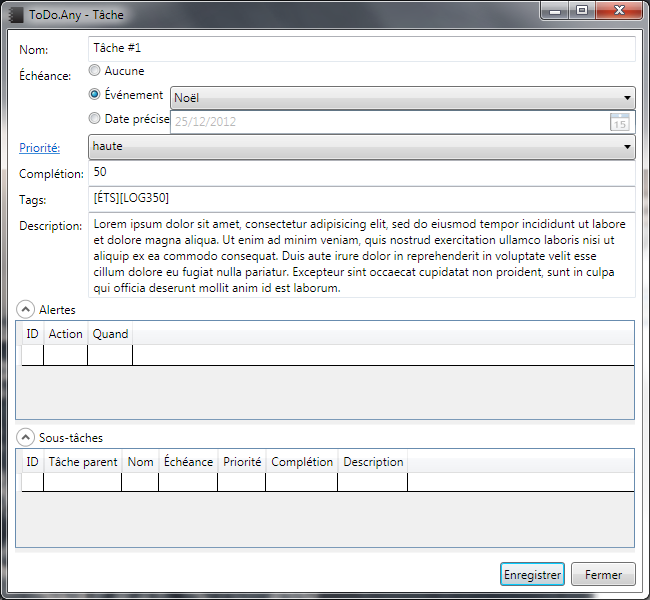
\includegraphics[width=1\textwidth]{fenetre_tache.png}
	\caption{Fenêtre concernant une tâche.}
\end{figure}

\newpage

\subsection{Priorités}

C'est à partir de cet écran que l'utilisateur peut faire la gestion des diverses priorités disponibles dans l'application. À la page 22 du document, dans l'annexe III, il y a de plus ample informations concernant cette fenetre.

\begin{figure}[H!]
	\centering
	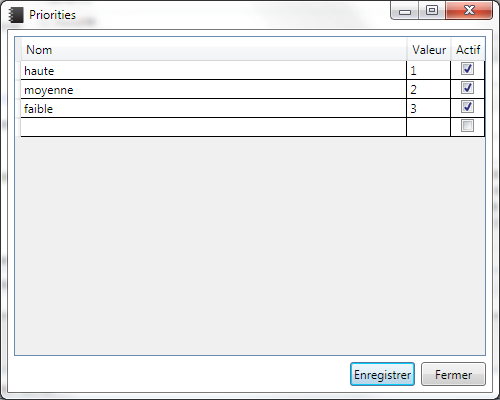
\includegraphics[width=1\textwidth]{fenetre_priorite.png}
	\caption{Fenêtre concernant les priorités.}
\end{figure}

\newpage

\section{Justification des choix de conception}

Divers patrons de conception ont été utilisé pour parvenir à la conception de l'application que nous avons présentement. 

Parmi les divers patrons disponibles, on compte le patron \emph{Many Workspaces} qui se retrouve à la fenêtre principale de l'application ou l'utilisateur à la possibilite d'avoir plusieurs listes d'ouvertes et de les organiser comme il veut via des onglets. L'utilisateur peut donc gérer plusieurs listes à la fois. 

Pour la navigation entre les fenêtres de l'application nous utilisons le patron \emph{Escape Hatch}. Ainsi, la navigation entre les fenêtres est limité et l'utilisateur peut toujours revenir a la fenêtre principale sans chercher pendant de longues minutes comment y revenir. Cela simplifie grandement l'interaction entre l'application et l'utilisateur en simplifiant le processus de navigation au maximum. 

Ensuite, pour ce qui est des listes, nous utilisons le patron \emph{Tree Table} sur, par exemple, la fenêtre principale. Avec ce patron, nous listons donc les tâches et chaque sous-tâche sous la tâche correspondante sous forme d'arborescence. Nous pouvons donc afficher un maximum d'information utile à l'utilisateur lorsque celui-ci le demande. Nous utilisons aussi le patron \emph{New-Item Row} dans la fenêtre Priorités pour permettre l'ajout rapide et infini de lignes dans le tableau sans que l'utilisateur n'ait besoin d'appuyer sur quoi que se soit. Pour ce qui est de toutes les grilles, le patron \emph{Sortable Table} s'applique et permet de trier l'information affiché en tout temps pour permettre à l'utilisateur de trouver ce qu'il veut plus rapidement. 

De plus, nous avons respecté le plus possible le contenu de la norme \emph{ISO 9241-120} à \emph{ISO 9241-129} qui traite sur les interactions sur les entrées et sorties.

Quelques changements on été effectué entre le prototype statique et dynamique. Parmi ces changements, on compte les options possibles pour une échéance dans la fenêtre sur les tâches. Ce changement a été fait à cause de limitations logiciels et par faute de temps. Il est à noter que ces changements n'influence en aucun cas l'efficacité de l'application.

\section{Améliorations possibles}

Quelques améliorations possibles seraient d'utiliser les lois psychomotrices de Fitts et Miller pour optimiser l'interface. Nous pourrions ainsi optimiser les déplacements que l'utilisateur doit faire avec sa souris pour cliquer sur les boutons et les champs de saisies dans les fenêtres. Mais, par faute de temps et de ressources humaines, il nous est donc impossible d'effectuer ces tests.

\chapter{Démonstration du prototype dynamique en laboratoire}

Un prototype dynamique de l'application est disponible à l'adresse suivante : \\
\url{https://github.com/xeph/LOG350.TP3}.

Évaluation du prototype en laboratoire  : le 4 décembre 2012 au laboratoire (pour les 2 groupes).

Exposé oral  : le 6 décembre 2012 dans un local à définir (pour les 2 groupes).

Remise du code final : le 11 décembre 2012 à 23h59 maximum par courriel à log350a2012@gmail.com.

Remise du rapport :  le 11 décembre 2012 à 23h59 maximum en version papier dans la chute du département.

Remise de la présentation de l’éxposé oral : le 6 décembre 2012 à 23h59 maximum par courriel à log350a2012@gmail.com .

\chapter{Tests avec utilisateurs}

\section{Méthodologie}

Avant d'effectuer les tests, un document expliquant la nature du projet et le déroulement des tests a été fourni aux utilisateurs. Les membres de l'équipe assument que le document a été lu lors de la rencontre. De plus, un formulaire de consentement sera obligatoirement signé par l'utilisateur et un membre de l'équipe pour que les deux parties s'entendent sur ce qui sera fait lors de la rencontre.

Pour faire les tests avec les utilisateurs, le ou les membres de l'équipe s'asseoiront avec l'utilisateur qui testera l'application. Par la suite, un membre de l'équipe se chargera de dire chaque tâche que l'utilisateur devra effectuer, et si l'utilisateur à des questions, il sera chargé de lui fournir les informations. Lorsque l'utilisateur aura terminé de faire une tâche, il y aura une brève pause pour que tout le monde ait le temps de prendre des notes. L'exécution de la tâche suivante se fera lorsque tout le monde aura terminer de prendre les notes pour la tâche courante. Quand toutes les tâches auront été exécuté, l'utilisateur pourra donner son opinion et ses impressions sur l'application sur des choses à améliorer, les points positifs et des fonctionnalitées qui pourraient être intéressante à ajouter.

Les tests se feront dans le calme et le respect. De plus, l'utilisateur peut, en tout temps, décider d'arrêter les tests sans devoir fournir une raison. Les données recueillis seront cependant conservé à moins que l'utilisateur ne demande à ce qu'elles soient détruites.

\newpage

\section{Liste des tâches}

\begin{table}
	\centering
	\begin{tabular}{|l|l|l|}
		\hline
		no Tache	& Titre et description		& Éléments que vous voulez vérifier et hypothèses 	\\ \hline 
		1		& Ajouter un événement		&  							\\ 
				& sans alertes.			&							\\ \hline
		2		& Modifier l'événement créer et	&							\\
				& ajouter une alerte.		&							\\ \hline
		3		& Ajouter le tag école		&							\\
				& à l'événement.			&							\\ \hline
		4		& Créer un événement et		&							\\
				& ajouter le tag travail.		&							\\ \hline
		5		& Rechercher les événements	& 							\\
				& par tag.				&							\\ \hline
		6		& Supprimer les événements	&							\\
				& contenant le tag travail.		&							\\ \hline
		7		& Trouver la fenêtre des		&							\\
				& priorités.				& 							\\ \hline
		8		& Ajouter une nouvelle priorité 	&							\\
				& valide.				&							\\ \hline
		9		& Désactiver une priorité ne	&							\\
				& contenant aucun événement ou &							\\
				& tâche associé.			&							\\ \hline
		10		& Ajouter plusieurs tâches		&							\\
				& (3-5 environ).			&							\\ \hline
		11		& Prendre une tâche et lui		&							\\
				& affecter 2 sous-tâches.		&							\\ \hline
		12		& Modifier la complétion d'une	&							\\
				& tâche non complété.		&							\\ \hline
		13		& Modifier la complétion de	&							\\
				& sous-tâches pour compléter	&							\\ 
				& une tâche.				&							\\ \hline
		14		& Supprimer une tâche complété.	&							\\ \hline
		15		& Modifier les informations		&							\\
				& d'une tâche non complété.	&							\\ \hline
		16		& Rechercher une tâche avec la 	&							\\
				& priorité créé précédement.	& 							\\ \hline
		17		& Créer un onglet comportant	&							\\
				& seulement les tâche concernant &							\\
				& l'école.				&							\\ \hline
	\end{tabular}
	\caption{Liste des tâches}
\end{table}

\section{Liste des utilisateurs}

Les caractéristiques principales des utilisateurs choisis sont la gestion de leurs tâches pour les travaux et devoirs au CEGEP ou bien à l'université et la gestion des rendez-vous pour les professionnels. Nous avons choisis ce nombre d'utilisateur, car il nous fallait un petit échantillon oeuvrant dans le même type de vie que le publique visée mais dans des sphères professionnelles différentes. Il est pertinant d'avoir testé avec ces utilisateurs parce que se sera principalement ce type d'utilisateur qui se servira d'une application comme celle-ci.

\newpage

\section{Résultats}

\begin{table}
	\centering
	\begin{tabular}{|l|l|l|}
	\hline
	no Tâche	& Points importants de l'observation	\\ \hline
	1		& 0						\\ \hline
	2		& 0						\\ \hline
	3		& 0						\\ \hline
	4		& 0						\\ \hline
	5		& 0						\\ \hline
	6		& 0						\\ \hline
	7		& 0						\\ \hline
	8		& 0						\\ \hline
	9		& 0						\\ \hline
	10		& 0						\\ \hline
	11		& 0						\\ \hline
	12		& 0						\\ \hline
	13		& 0						\\ \hline
	14		& 0						\\ \hline
	15		& 0						\\ \hline
	16		& 0						\\ \hline
	17		& 0						\\ \hline
	\end{tabular}
	\caption{Résultats de l'utilisateur 1}
\end{table}

\newpage

\begin{table}
	\centering
	\begin{tabular}{|l|l|l|}
	\hline
	no Tâche	& Points importants de l'observation	\\ \hline
	1		& 0						\\ \hline
	2		& 0						\\ \hline
	3		& 0						\\ \hline
	4		& 0						\\ \hline
	5		& 0						\\ \hline
	6		& 0						\\ \hline
	7		& 0						\\ \hline
	8		& 0						\\ \hline
	9		& 0						\\ \hline
	10		& 0						\\ \hline
	11		& 0						\\ \hline
	12		& 0						\\ \hline
	13		& 0						\\ \hline
	14		& 0						\\ \hline
	15		& 0						\\ \hline
	16		& 0						\\ \hline
	17		& 0						\\ \hline
	\end{tabular}
	\caption{Résultats de l'utilisateur 2}
\end{table}

\newpage

\begin{table}
	\centering
	\begin{tabular}{|l|l|l|}
	\hline
	no Tâche	& Points importants de l'observation	\\ \hline
	1		& 0						\\ \hline
	2		& 0						\\ \hline
	3		& 0						\\ \hline
	4		& 0						\\ \hline
	5		& 0						\\ \hline
	6		& 0						\\ \hline
	7		& 0						\\ \hline
	8		& 0						\\ \hline
	9		& 0						\\ \hline
	10		& 0						\\ \hline
	11		& 0						\\ \hline
	12		& 0						\\ \hline
	13		& 0						\\ \hline
	14		& 0						\\ \hline
	15		& 0						\\ \hline
	16		& 0						\\ \hline
	17		& 0						\\ \hline
	\end{tabular}
	\caption{Résultats de l'utilisateur 3}
\end{table}

\newpage

\section{Discussion et recommandations}

\begin{table}
	\centering
	\begin{tabular}{|l|l|l|}
	\hline
	no Tâche	& Résumé	& Recommandation 	\\ \hline
	1		& 0		& 0 			\\ \hline
	2		& 0		& 0 			\\ \hline
	3		& 0		& 0 			\\ \hline
	4		& 0		& 0 			\\ \hline
	5		& 0		& 0 			\\ \hline
	6		& 0		& 0 			\\ \hline
	7		& 0		& 0 			\\ \hline
	8		& 0		& 0 			\\ \hline
	9		& 0		& 0 			\\ \hline
	10		& 0		& 0 			\\ \hline
	11		& 0		& 0 			\\ \hline
	12		& 0		& 0 			\\ \hline
	13		& 0		& 0 			\\ \hline
	14		& 0		& 0 			\\ \hline
	15		& 0		& 0 			\\ \hline
	16		& 0		& 0 			\\ \hline
	\end{tabular}
	\caption{Recommandations par les observateurs}
\end{table}

\begin{table}
	\centering
	\begin{tabular}{|l|l|l|}
	\hline
	no Tâche	& Résumé	& Recommandation 	\\ \hline
	1		& 0		& 0 			\\ \hline
	2		& 0		& 0 			\\ \hline
	3		& 0		& 0 			\\ \hline
	4		& 0		& 0 			\\ \hline
	5		& 0		& 0 			\\ \hline
	6		& 0		& 0 			\\ \hline
	7		& 0		& 0 			\\ \hline
	8		& 0		& 0 			\\ \hline
	9		& 0		& 0 			\\ \hline
	10		& 0		& 0 			\\ \hline
	11		& 0		& 0 			\\ \hline
	12		& 0		& 0 			\\ \hline
	13		& 0		& 0 			\\ \hline
	14		& 0		& 0 			\\ \hline
	15		& 0		& 0 			\\ \hline
	16		& 0		& 0 			\\ \hline
	\end{tabular}
	\caption{Recommandations par les utilisateurs}
\end{table}

\chapter{Changements recommandés}

DUMMY DATA

\begin{enumerate}
	\item Fournir un menu affichant les actions possibles sur un endroit precis de l'application.
	\item Fournir un menu d'aide (tooltip par exemple) explicant diverses fonctionnalites qui ne sont pas toujours evidente pour l'utilisateur, comme le systeme de tag.
	\item Changer le champ completion dans la fenetre tache pour un slider, comme sa l'utilisateur ne pourra pas entrer ce qu'il veut.
	\item Remplacer le systeme de criteres de la recherche pour le rendre moins lourd a utiliser. Comme par exemple un systeme de recherche
	\item Fournir un interface offrant des parametres de base comme un champ adresse email par defaut pour les alertes par exemple.
	\item Fournir un moyen de bien identifier les onglets ne pouvant etre ferme sur la fenetre principale.
	\item Lors de l'ouverture d'un element de l'arbre les autres elements ouverts du meme niveau d'imbrication se ferment automatiquement pour sauver de l'espace.
\end{enumerate}

\chapter{Conclusion}

En conclusion, ce qui ressort du projet est qu'il peut être très difficile et complexe de concevoir un interface facile d'utilisation tout en étant efficace. Il existe divers patrons et diverses normes nous aidant à parvenir à cette fin et il faut savoir faire les bonnes combinaisons pour arriver à un résultat satisfaisant. 

Les différentes étapes ont eu comme impact, sur la qualité du produit final, les points suivants :

\begin{itemize}
	\item Impossible d'évaluer la complexité de l'implémantation de l'interface sans ecrire le code pour la faire fonctionner.
	\item Définis tous les interfaces et les buts accomplis par chacun avant de penser à écrire une seule ligne de code.
\end{itemize}

Il reste a faire \dots

Nous avons tiré comme lecons qu'il vaut mieux voir si l'implémentation de la fenêtre est possible dans le temps alloué avec les ressources humaines disponibles avant de figer dans le béton un interface de l'application. De plus, pour tout ce qui attrait à l'apparence de l'application, il vaut mieux faire appel à un designer spécialisé dans le domaine plutôt que d'essayer de faire quelque chose par nous même qui ne donnera pas un beau rendu visuel.

Nous recommandons que le contenu du cours s'applique plus au projet, car, souvent, il est difficile d'établir des liens entre la matière présentée en classe et les laboratoires que nous effectuons. Par exemple, les liens entre le SDK pour iPhone et notre projet en C\#/WPF sont inexistants ou bien les techniques et styles d'interactions peuvent etre difficile à appliquer selon les contextes des divers projets des étudiants.

\appendix
\multiannexe

\chapter{Formulaire de consentement des utilisateurs}


\includepdf[pages=-]{form.pdf}

\chapter{Document de présentation du projet}

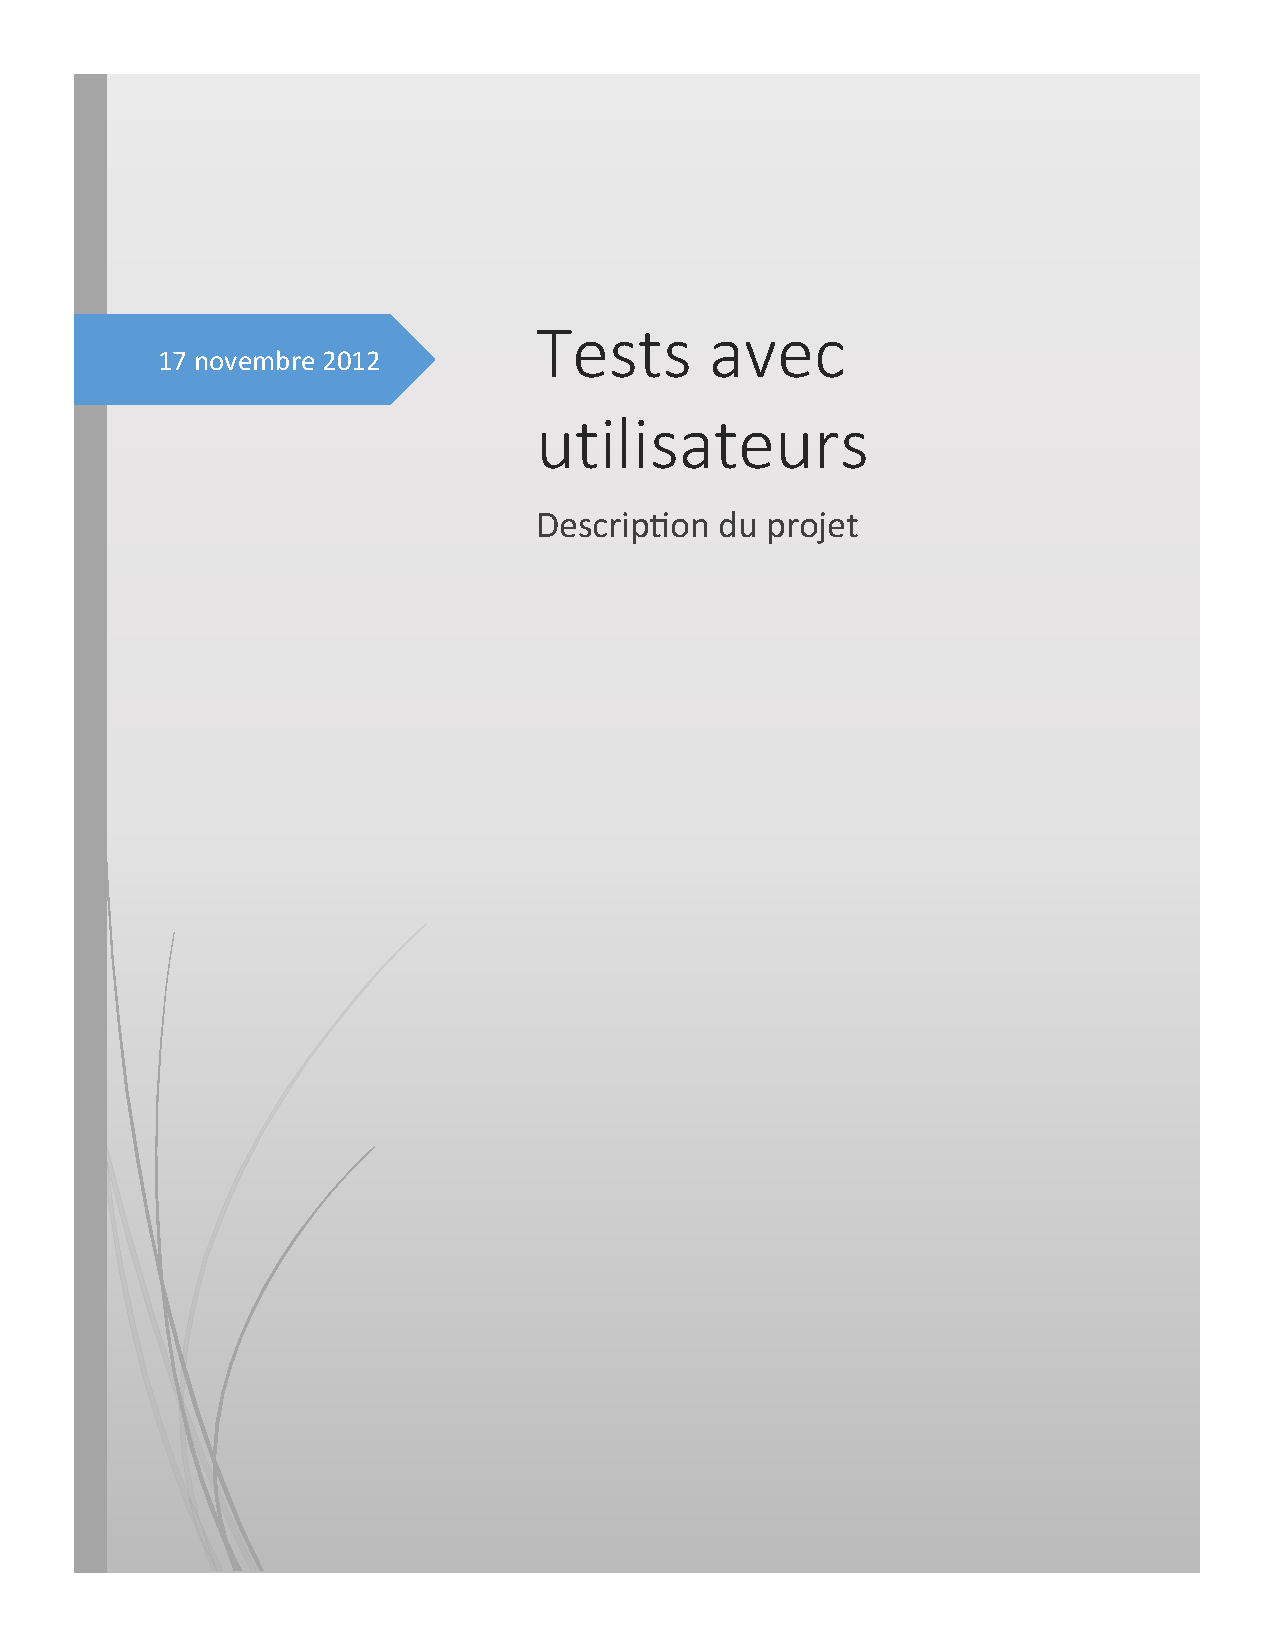
\includepdf[pages=-]{document.pdf}

\chapter{Travail Pratique 2}

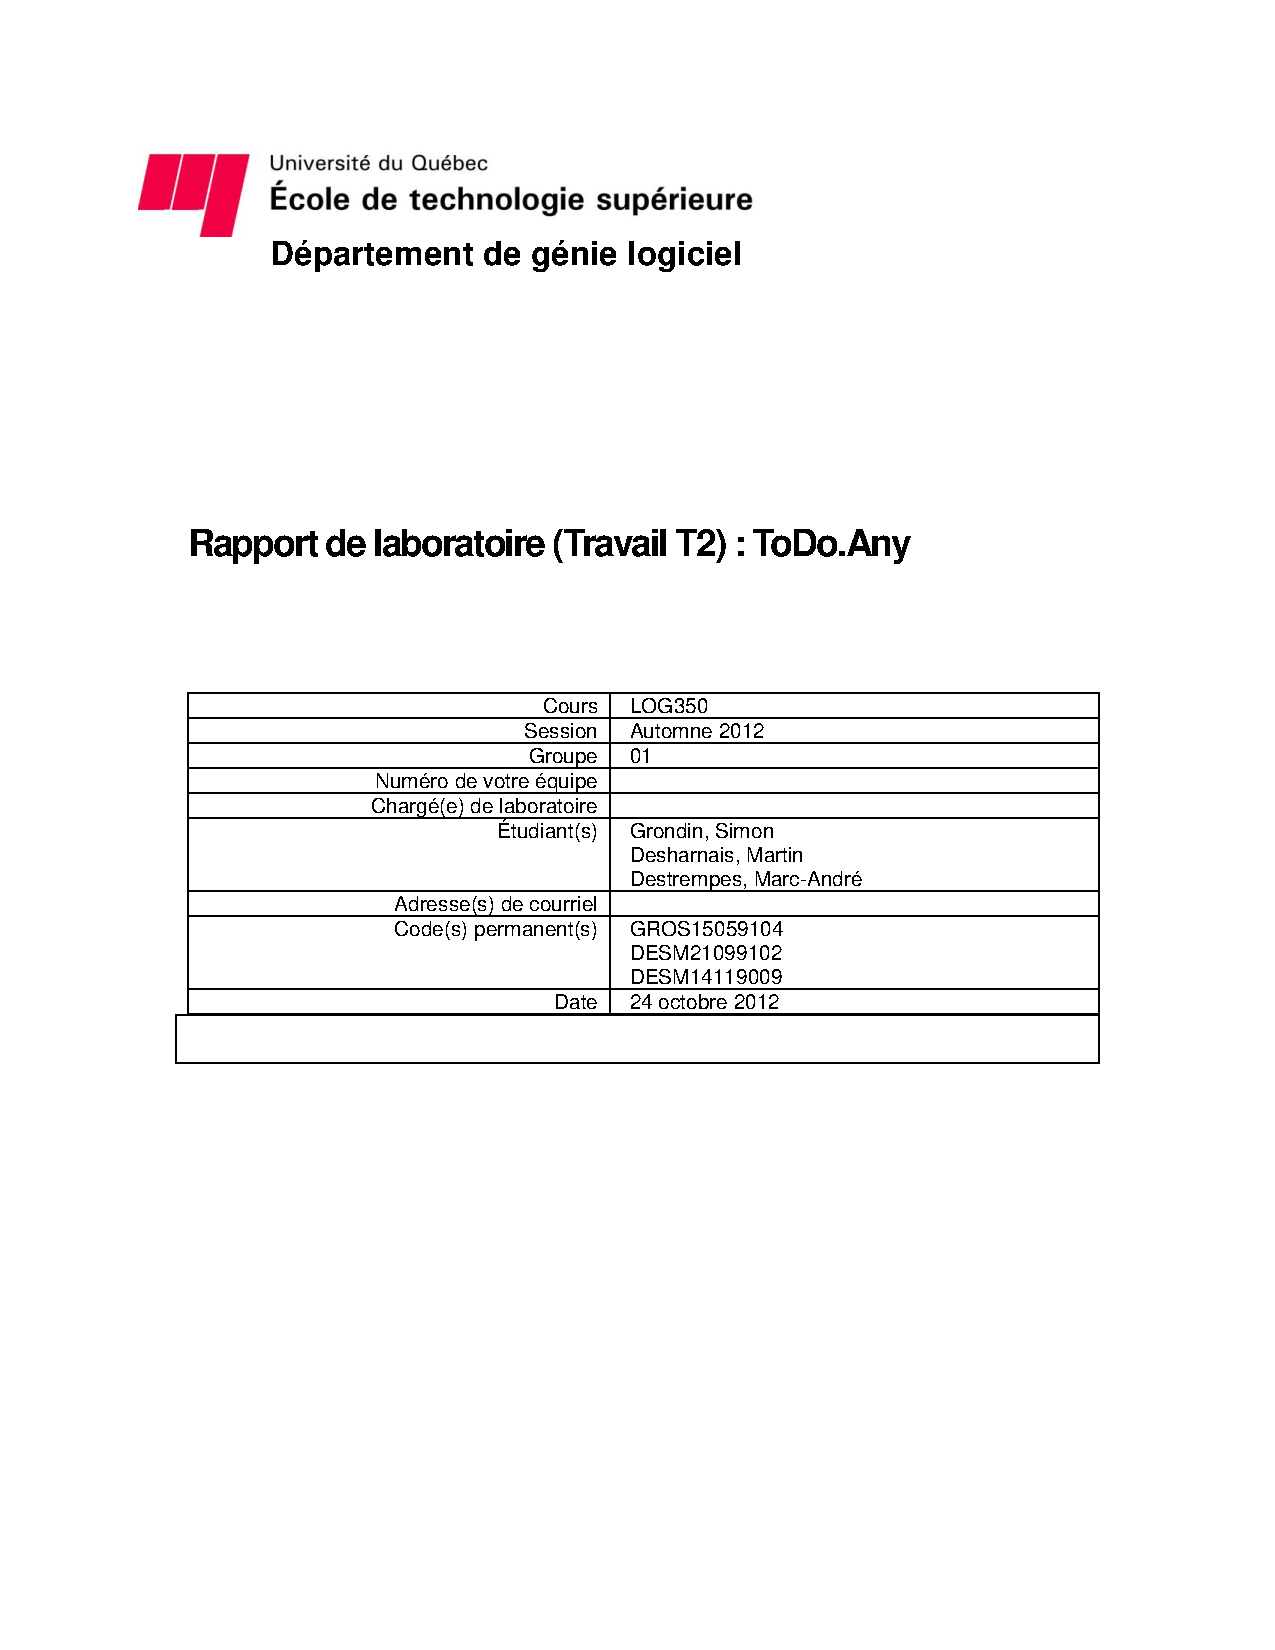
\includepdf[pages=-]{T2.pdf}

\end{document}
